\section{Planeación de acciones}

\begin{frame}
  \Huge
  Planeación de acciones
\end{frame}

\begin{frame}\frametitle{Máquinas de estados finitas}
  Las FSM son modelos que permiten representar procesos discretos donde el sistema puede estar en un estado bien definido y existen un conjunto de reglas para definir el estado siguiente en función del estado actual y las entradas. Opcionalmente, se pueden definir salidas para cada estado. \\
  Formalmente, una FSM está definida por:
  \begin{itemize}
  \item $S$ : Conjunto finito no vacío de estados
  \item $\Sigma$ : Conjunto finito no vacío de entradas
  \item $s_0 \in S$ : Estado inicial
  \item $\delta : S\times\Sigma\rightarrow S$ : Función de transición de estados
  \item $F$ : Conjunto de estados finales (puede ser un conjunto vacío)
  \end{itemize}
\end{frame}

\begin{frame}\frametitle{Carta ASM}
  Una forma de representar los estados y transiciones de una FSM es mediante una carta ASM. Ejemplo:
  \begin{figure}
    \centering
    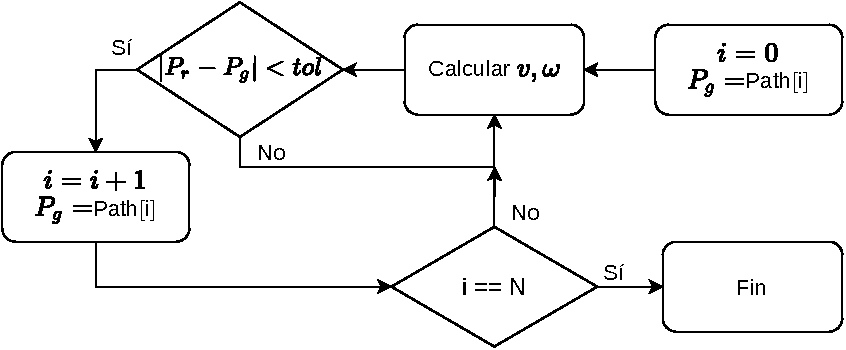
\includegraphics[width=0.6\textwidth]{Figures/PathFollowing.pdf}
  \end{figure}
  Las máquinas de estados se pueden utiizar para ejecutar tareas ``sencillas'' en un robot de servicio doméstico. 
\end{frame}

\begin{frame}\frametitle{FSM para manipular objetos}
  En cada estado podemos enviar comandos de movimiento y utilizar resultados de percepción para definir el siguiente estado:
  \begin{figure}
    \centering
    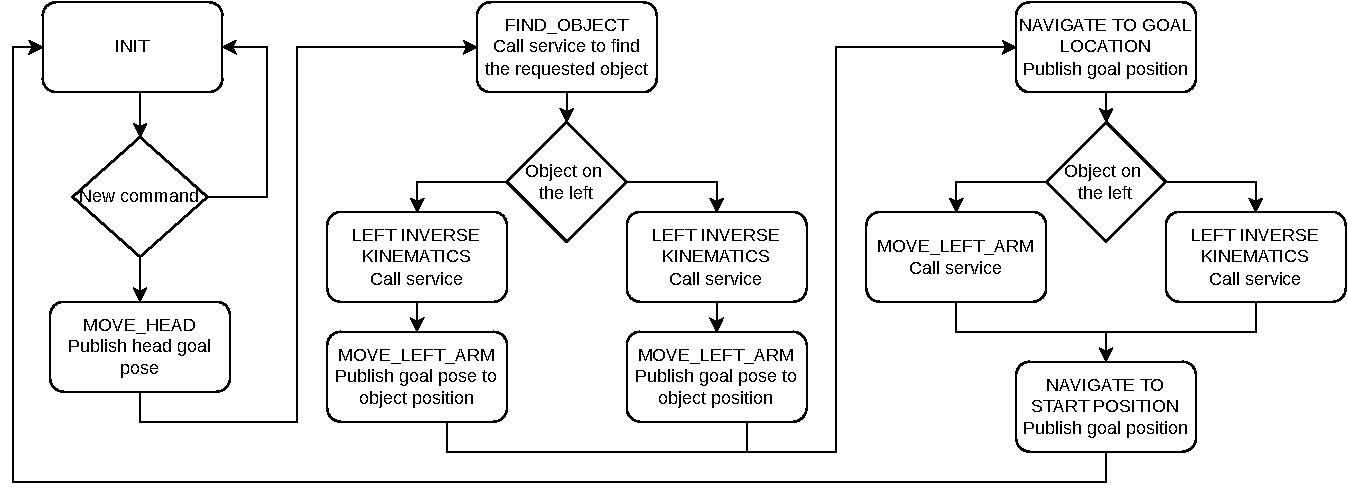
\includegraphics[width=\textwidth]{Figures/FSM.pdf}
  \end{figure}
\end{frame}

\begin{frame}[containsverbatim]\frametitle{Ejercicio Final}
  Abra el archivo \texttt{catkin\_ws/src/exercises/scripts/simple\_service\_robot.py} e inspeccione los diversos estados. Ejecute el comando:
  \begin{lstlisting}
    roslaunch bring_up final_exercise.launch
  \end{lstlisting}
  Y en otra terminal, corra la plneación para un robot de servicio simple:
  \begin{lstlisting}
    rosrun exercises simple_service_robot.py
  \end{lstlisting}
\end{frame}
